%%
%% Automatically generated file from DocOnce source
%% (https://github.com/hplgit/doconce/)
%%

% #define PREAMBLE

% #ifdef PREAMBLE
%-------------------- begin preamble ----------------------

\documentclass[%
oneside,                 % oneside: electronic viewing, twoside: printing
final,                   % draft: marks overfull hboxes, figures with paths
10pt,french]{article}

\listfiles               %  print all files needed to compile this document

\usepackage{relsize,makeidx,color,setspace,amsmath,amsfonts,amssymb}
\usepackage[table]{xcolor}
\usepackage{bm,ltablex,microtype}

\usepackage[pdftex]{graphicx}

% Movies are handled by the href package
\newenvironment{doconce:movie}{}{}
\newcounter{doconce:movie:counter}


% Packages for typesetting blocks of computer code
\usepackage{fancyvrb,framed,moreverb}

% Define colors
\definecolor{orange}{cmyk}{0,0.4,0.8,0.2}
\definecolor{tucorange}{rgb}{1.0,0.64,0}
\definecolor{darkorange}{rgb}{.71,0.21,0.01}
\definecolor{darkgreen}{rgb}{.12,.54,.11}
\definecolor{myteal}{rgb}{.26, .44, .56}
\definecolor{gray}{gray}{0.45}
\definecolor{mediumgray}{gray}{.8}
\definecolor{lightgray}{gray}{.95}
\definecolor{brown}{rgb}{0.54,0.27,0.07}
\definecolor{purple}{rgb}{0.5,0.0,0.5}
\definecolor{darkgray}{gray}{0.25}
\definecolor{darkblue}{rgb}{0,0.08,0.45}
\definecolor{darkblue2}{rgb}{0,0,0.8}
\definecolor{lightred}{rgb}{1.0,0.39,0.28}
\definecolor{lightgreen}{rgb}{0.48,0.99,0.0}
\definecolor{lightblue}{rgb}{0.53,0.81,0.92}
\definecolor{lightblue2}{rgb}{0.3,0.3,1.0}
\definecolor{lightpurple}{rgb}{0.87,0.63,0.87}
\definecolor{lightcyan}{rgb}{0.5,1.0,0.83}

\colorlet{comment_green}{green!50!black}
\colorlet{string_red}{red!60!black}
\colorlet{keyword_pink}{magenta!70!black}
\colorlet{indendifier_green}{green!70!white}

% Backgrounds for code
\definecolor{cbg_gray}{rgb}{.95, .95, .95}
\definecolor{bar_gray}{rgb}{.92, .92, .92}

\definecolor{cbg_yellowgray}{rgb}{.95, .95, .85}
\definecolor{bar_yellowgray}{rgb}{.95, .95, .65}

\colorlet{cbg_yellow2}{yellow!10}
\colorlet{bar_yellow2}{yellow!20}

\definecolor{cbg_yellow1}{rgb}{.98, .98, 0.8}
\definecolor{bar_yellow1}{rgb}{.98, .98, 0.4}

\definecolor{cbg_red1}{rgb}{1, 0.85, 0.85}
\definecolor{bar_red1}{rgb}{1, 0.75, 0.85}

\definecolor{cbg_blue1}{rgb}{0.87843, 0.95686, 1.0}
\definecolor{bar_blue1}{rgb}{0.7,     0.95686, 1}

%\setlength{\fboxsep}{-1.5mm}  % adjust cod_vpad/pro_vpad background box

%% Background for code blocks (parameter is color name)

%% pro/cod_vpad: gives some vertical padding before and after the text
%% (but has more simplistic code than _cod/pro_tight+cod/pro).
%% pro/cod_vpad can be used to enclose Verbatim or lst begin/end for code.
%% pro/cod calls _pro/cod_tight and has very little vertical padding,
%% used to enclose Verbatim and other begin/end for code.
%% (pro/cod is what the ptex2tex program could produce with the
%% Blue/BlueBar definitions in .ptex2tex.cfg.)

\newenvironment{cod_vpad}[1]{
   \def\FrameCommand{\colorbox{#1}}
   \MakeFramed{\FrameRestore}}
   {\endMakeFramed}

\newenvironment{_cod_tight}[1]{
   \def\FrameCommand{\colorbox{#1}}
   \FrameRule0.6pt\MakeFramed {\FrameRestore}\vskip3mm}
   {\vskip0mm\endMakeFramed}

\newenvironment{cod}[1]{
\bgroup\rmfamily
\fboxsep=0mm\relax
\begin{_cod_tight}{#1}
\list{}{\parsep=-2mm\parskip=0mm\topsep=0pt\leftmargin=2mm
\rightmargin=2\leftmargin\leftmargin=4pt\relax}
\item\relax}
{\endlist\end{_cod_tight}\egroup}

%% Background for complete program blocks (parameter 1 is color name
%% for background, parameter 2 is color for left bar)
\newenvironment{pro_vpad}[2]{
   \def\FrameCommand{\color{#2}\vrule width 1mm\normalcolor\colorbox{#1}}
   \MakeFramed{\FrameRestore}}
   {\endMakeFramed}

\newenvironment{_pro_tight}[2]{
   \def\FrameCommand{\color{#2}\vrule width 1mm\normalcolor\colorbox{#1}}
   \FrameRule0.6pt\MakeFramed {\advance\hsize-2mm\FrameRestore}\vskip3mm}
   {\vskip0mm\endMakeFramed}

\newenvironment{pro}[2]{
\bgroup\rmfamily
\fboxsep=0mm\relax
\begin{_pro_tight}{#1}{#2}
\list{}{\parsep=-2mm\parskip=0mm\topsep=0pt\leftmargin=2mm
\rightmargin=2\leftmargin\leftmargin=4pt\relax}
\item\relax}
{\endlist\end{_pro_tight}\egroup}

\usepackage{minted}
\usemintedstyle{default}

\usepackage[T1]{fontenc}
%\usepackage[latin1]{inputenc}
\usepackage{ucs}
\usepackage[utf8x]{inputenc}

\usepackage{lmodern}         % Latin Modern fonts derived from Computer Modern

% Hyperlinks in PDF:
\definecolor{linkcolor}{rgb}{0,0,0.4}
\usepackage{hyperref}
\hypersetup{
    breaklinks=true,
    colorlinks=true,
    linkcolor=linkcolor,
    urlcolor=linkcolor,
    citecolor=black,
    filecolor=black,
    %filecolor=blue,
    pdfmenubar=true,
    pdftoolbar=true,
    bookmarksdepth=3   % Uncomment (and tweak) for PDF bookmarks with more levels than the TOC
    }
%\hyperbaseurl{}   % hyperlinks are relative to this root

\setcounter{tocdepth}{2}  % levels in table of contents

% Tricks for having figures close to where they are defined:
% 1. define less restrictive rules for where to put figures
\setcounter{topnumber}{2}
\setcounter{bottomnumber}{2}
\setcounter{totalnumber}{4}
\renewcommand{\topfraction}{0.95}
\renewcommand{\bottomfraction}{0.95}
\renewcommand{\textfraction}{0}
\renewcommand{\floatpagefraction}{0.75}
% floatpagefraction must always be less than topfraction!
% 2. ensure all figures are flushed before next section
\usepackage[section]{placeins}
% 3. enable begin{figure}[H] (often leads to ugly pagebreaks)
%\usepackage{float}\restylefloat{figure}

% --- fancyhdr package for fancy headers ---
\usepackage{fancyhdr}
\fancyhf{} % sets both header and footer to nothing
\renewcommand{\headrulewidth}{0pt}
\fancyfoot[LE,RO]{\thepage}
% Ensure copyright on titlepage (article style) and chapter pages (book style)
\fancypagestyle{plain}{
  \fancyhf{}
  \fancyfoot[C]{{\footnotesize \copyright\ 2019, Ahmed Ammar. Released under CC Attribution 4.0 license}}
%  \renewcommand{\footrulewidth}{0mm}
  \renewcommand{\headrulewidth}{0mm}
}
% Ensure copyright on titlepages with \thispagestyle{empty}
\fancypagestyle{empty}{
  \fancyhf{}
  \fancyfoot[C]{{\footnotesize \copyright\ 2019, Ahmed Ammar. Released under CC Attribution 4.0 license}}
  \renewcommand{\footrulewidth}{0mm}
  \renewcommand{\headrulewidth}{0mm}
}

\pagestyle{fancy}


\usepackage{framed,wrapfig}

% --- begin definitions of admonition environments ---

% Admonition style "grayicon" has colored background, no frame, and an icon
% Admon "notice"
\definecolor{grayicon_notice_background}{rgb}{0.91,0.91,0.91}
% \fboxsep sets the space between the text and the box
\newenvironment{noticeshaded}
{\def\FrameCommand{\fboxsep=3mm\colorbox{grayicon_notice_background}}
 \MakeFramed {\advance\hsize-\width \FrameRestore}}{\endMakeFramed}

\newenvironment{notice_grayiconadmon}[1][Notice]{
\begin{noticeshaded}
\noindent
\begin{wrapfigure}{l}{0.07\textwidth}
\vspace{-13pt}

\includegraphics[width=0.07\textwidth]{latex_figs/small_gray_notice}
\end{wrapfigure} \textbf{#1}\par
\nobreak\noindent\ignorespaces
}
{
\end{noticeshaded}
}

% Admonition style "grayicon" has colored background, no frame, and an icon
% Admon "summary"
\definecolor{grayicon_summary_background}{rgb}{0.91,0.91,0.91}
% \fboxsep sets the space between the text and the box
\newenvironment{summaryshaded}
{\def\FrameCommand{\fboxsep=3mm\colorbox{grayicon_summary_background}}
 \MakeFramed {\advance\hsize-\width \FrameRestore}}{\endMakeFramed}

\newenvironment{summary_grayiconadmon}[1][Summary]{
\begin{summaryshaded}
\noindent
\begin{wrapfigure}{l}{0.07\textwidth}
\vspace{-13pt}
\includegraphics[width=0.07\textwidth]{latex_figs/small_gray_summary}
\end{wrapfigure} \textbf{#1}\par
\nobreak\noindent\ignorespaces
}
{
\end{summaryshaded}
}

% Admonition style "grayicon" has colored background, no frame, and an icon
% Admon "warning"
\definecolor{grayicon_warning_background}{rgb}{0.91,0.91,0.91}
% \fboxsep sets the space between the text and the box
\newenvironment{warningshaded}
{\def\FrameCommand{\fboxsep=3mm\colorbox{grayicon_warning_background}}
 \MakeFramed {\advance\hsize-\width \FrameRestore}}{\endMakeFramed}

\newenvironment{warning_grayiconadmon}[1][Warning]{
\begin{warningshaded}
\noindent
\begin{wrapfigure}{l}{0.07\textwidth}
\vspace{-13pt}
\includegraphics[width=0.07\textwidth]{latex_figs/small_gray_warning}
\end{wrapfigure} \textbf{#1}\par
\nobreak\noindent\ignorespaces
}
{
\end{warningshaded}
}

% Admonition style "grayicon" has colored background, no frame, and an icon
% Admon "question"
\definecolor{grayicon_question_background}{rgb}{0.91,0.91,0.91}
% \fboxsep sets the space between the text and the box
\newenvironment{questionshaded}
{\def\FrameCommand{\fboxsep=3mm\colorbox{grayicon_question_background}}
 \MakeFramed {\advance\hsize-\width \FrameRestore}}{\endMakeFramed}

\newenvironment{question_grayiconadmon}[1][Question]{
\begin{questionshaded}
\noindent
\begin{wrapfigure}{l}{0.07\textwidth}
\vspace{-13pt}
\includegraphics[width=0.07\textwidth]{latex_figs/small_gray_question2}
\end{wrapfigure} \textbf{#1}\par
\nobreak\noindent\ignorespaces
}
{
\end{questionshaded}
}

% Admonition style "grayicon" has colored background, no frame, and an icon
% Admon "block"
\definecolor{grayicon_block_background}{rgb}{0.91,0.91,0.91}
% \fboxsep sets the space between the text and the box
\newenvironment{blockshaded}
{\def\FrameCommand{\fboxsep=3mm\colorbox{grayicon_block_background}}
 \MakeFramed {\advance\hsize-\width \FrameRestore}}{\endMakeFramed}

\newenvironment{block_grayiconadmon}[1][Block]{
\begin{blockshaded}
\noindent
 \textbf{#1}\par
\nobreak\noindent\ignorespaces
}
{
\end{blockshaded}
}

% --- end of definitions of admonition environments ---

% prevent orhpans and widows
\clubpenalty = 10000
\widowpenalty = 10000

% --- end of standard preamble for documents ---


\usepackage[french]{babel}

% insert custom LaTeX commands...

\raggedbottom
\makeindex
\usepackage[totoc]{idxlayout}   % for index in the toc
\usepackage[nottoc]{tocbibind}  % for references/bibliography in the toc

%-------------------- end preamble ----------------------

\begin{document}

% matching end for #ifdef PREAMBLE
% #endif

\newcommand{\exercisesection}[1]{\subsection*{#1}}


% ------------------- main content ----------------------



% ----------------- title -------------------------

\title{Développer des applications de bureau avec Python et Qt}

% ----------------- author(s) -------------------------

\author{Ahmed Ammar\footnote{Email: \texttt{ahmed.ammar@fst.utm.tn}. Faculté des Sciences de Tunis, Université de Tunis El Manar.}}

% ----------------- end author(s) -------------------------

\date{Mar 7, 2019}
\maketitle

\tableofcontents


\vspace{1cm} % after toc




% !split
\section{Introduction}
Dans ce chapitre, nous allons passer à la création d’applications graphiques. De telles applications permettent de modifier l'apparence d'un programme en utilisant des \textbf{éléments de contrôle} tels que des \textbf{widgets}, des \textbf{boutons}, des \textbf{curseurs}, etc.

\textbf{PyQt5} (\href{{https://www.riverbankcomputing.com/software/pyqt/intro}}{\nolinkurl{https://www.riverbankcomputing.com/software/pyqt/intro}}) est une boîte à outils de widgets d' interface graphique (en anglais \textbf{GUI} pour \emph{Graphical User Interface}) combinant le langage de programmation Python et le logiciel \textbf{Qt5} (\href{{https://www.qt.io}}{\nolinkurl{https://www.qt.io}}). PyQt5 est une bibliothèque d'interface graphique populaire qui présente de nombreux avantages par rapport aux autres bibliothèques d'interface graphique telles que \emph{Tkinter} et \emph{wx}. Ceux-ci inclus:

\begin{itemize}
\item Bibliothèque d'interface graphique multi-plateforme (Windows, MacOS, Linux).

\item Bonne performance.

\item Prise en charge des styles personnalisés.

\item Plus de bibliothèques pour la conception d'interface graphique complexe.

\item Facilité d'utilisation.
\end{itemize}

\noindent
\section{Premières étapes pour la création d'une application graphique à l'aide de PyQt5}

\subsection{Importation de PyQt5 et création d'une "fenêtre PyQt5"}

Passons directement à l'action et apprenons à créer une fenêtre simple avec PyQt5. Premièrement, nous devrons importer certains modules essentiels à l’exécution d’une interface graphique avec PyQt5. Nous commençons par \textbf{importer} quelques sous-modules de PyQt5.

\begin{cod}{cbg_gray}\begin{minted}[fontsize=\fontsize{9pt}{9pt},linenos=false,mathescape,baselinestretch=1.0,fontfamily=tt,xleftmargin=2mm]{python}
from PyQt5.QtWidgets import QApplication, QWidget
\end{minted}
\end{cod}
\noindent

\begin{notice_grayiconadmon}[Notice]
\texttt{QtWidgets} est l'un des nombreux composants de PyQt5. Certains des plus couramment utilisés sont énumérés ci-dessous:
\begin{itemize}
\item \texttt{QtWidgets}: Contient des classes qui fournissent un ensemble d'éléments pour créer une interface graphique classique de type bureau.

\item \texttt{QtCore}: Ce module contient les classes principales, y compris la boucle d'événement et les mécanismes \texttt{signal} et \texttt{slot} de Qt.

\item \texttt{QtGui}: Celui-ci contient des classes pour l’intégration du système de fenêtrage, la gestion des événements, les graphiques 2D, les images de base, les polices et le texte.

\item \texttt{QtDesigner}: Ce module contient des classes permettant l'extension de \emph{Qt Designer} à l'aide de PyQt5.

\item \texttt{uic}: Ce module contient des classes permettant de gérer les fichiers \textbf{.ui} créés par Qt Designer décrivant l’ensemble ou une partie d’une interface graphique.

\item etc.
\end{itemize}

\noindent
\end{notice_grayiconadmon} % title: Notice



Ensuite, nous importons le module \texttt{sys} car nous voulons accéder aux arguments de ligne de commande. Ceux-ci sont contenus dans la liste `sys.argv

\begin{cod}{cbg_gray}\begin{minted}[fontsize=\fontsize{9pt}{9pt},linenos=false,mathescape,baselinestretch=1.0,fontfamily=tt,xleftmargin=2mm]{python}
import sys
app = QApplication(sys.argv)
\end{minted}
\end{cod}
\noindent

En utilisant les arguments de ligne de commande contenus dans \texttt{sys.argv}, nous devrions créer un objet \texttt{QApplication}. Dans l'exemple ci-dessus, nous avons enregistré cet objet sous le nom \textbf{app}. Ceci est l'objet \emph{exécuté} lorsque nous exécutons à l'invite de commande la commande \texttt{python filename.py} où \textbf{filename.py} est le fichier dans lequel les instructions sont stockées. Cet objet contiendra tous les éléments de l'interface graphique et leurs méthodes. Par conséquent, lorsque cet objet est créé et \emph{exécuté}, nous avons accès à toutes les interfaces graphiques utilisées dans le programme. Les éléments de l'interface graphique sont hérités de la classe \texttt{QWidgets}. Nous obtenons donc un objet \texttt{QWidget} comme indiqué ci-dessous.
\begin{cod}{cbg_gray}\begin{minted}[fontsize=\fontsize{9pt}{9pt},linenos=false,mathescape,baselinestretch=1.0,fontfamily=tt,xleftmargin=2mm]{python}
window = QWidget()
\end{minted}
\end{cod}
\noindent
En utilisant les nombreuses méthodes \emph{set}, nous pouvons définir les valeurs des différents attributs de cet objet \emph{window}. Nous allons d’abord définir les dimensions de la fenêtre en utilisant la méthode \texttt{setGeometry}. Il prend quatre paramètres: \textbf{x} coordonnée du point le plus à gauche de l'objet (\emph{window}), \textbf{y} coordonnée du point le plus haut, \textbf{la largeur} et \textbf{la hauteur} de la fenêtre, dans cet ordre. Toutes ces valeurs doivent être des entiers référencés par rapport aux coordonnées d'écran natives. Par exemple, nous pourrions écrire:

\begin{cod}{cbg_gray}\begin{minted}[fontsize=\fontsize{9pt}{9pt},linenos=false,mathescape,baselinestretch=1.0,fontfamily=tt,xleftmargin=2mm]{python}
window.setGeometry(400, 100, 300, 200)
\end{minted}
\end{cod}
\noindent
Cela définirait la fenêtre avec une largeur de 300 pixels et une hauteur de 200 pixels à 400 pixels du côté gauche et à 100 pixels du haut de l'écran natif (écran de votre ordinateur).

Nous pouvons définir un titre pour la fenêtre. Par exemple:

\begin{cod}{cbg_gray}\begin{minted}[fontsize=\fontsize{9pt}{9pt},linenos=false,mathescape,baselinestretch=1.0,fontfamily=tt,xleftmargin=2mm]{python}
window.setWindowTitle('My first app')
\end{minted}
\end{cod}
\noindent
afficherait \emph{My first app} dans la barre de titre de la fenêtre.

Une fois que nous sommes satisfaits de l'interface graphique que nous avons construite, nous appelons:
\begin{cod}{cbg_gray}\begin{minted}[fontsize=\fontsize{9pt}{9pt},linenos=false,mathescape,baselinestretch=1.0,fontfamily=tt,xleftmargin=2mm]{python}
window.show()
\end{minted}
\end{cod}
\noindent

pour afficher l'objet graphique dans \emph{l'application} que nous avons créée. Cependant, l'application n'est toujours pas exécutée. Pour exécuter l'application, nous exécutons la commande:
\begin{cod}{cbg_gray}\begin{minted}[fontsize=\fontsize{9pt}{9pt},linenos=false,mathescape,baselinestretch=1.0,fontfamily=tt,xleftmargin=2mm]{python}
app.exec()
\end{minted}
\end{cod}
\noindent
La méthode \texttt{.show ()} est une méthode QT qui ouvre la fenêtre à l'écran pour l'utilisateur.

Enfin, pour assurer une fermeture agréable et propre de l'application lorsque nous quittons:
\begin{cod}{cbg_gray}\begin{minted}[fontsize=\fontsize{9pt}{9pt},linenos=false,mathescape,baselinestretch=1.0,fontfamily=tt,xleftmargin=2mm]{python}
sys.exit(app.exec_())
\end{minted}
\end{cod}
\noindent
Le code complet de cette application est donné ci-dessous et le résultat est illustré à la Figure~\ref{fig:myfirstapp}. Le code peut être stocké dans un fichier, par exemple \textbf{myfirstapp.py}, puis lorsque vous exécutez la commande \texttt{python MyFirstApp.py} à l'invite de commande (ou dans Spyder), vous obtenez la fenêtre de sortie affichée.

\begin{pro}{cbg_gray}{bar_gray}\begin{minted}[fontsize=\fontsize{9pt}{9pt},linenos=false,mathescape,baselinestretch=1.0,fontfamily=tt,xleftmargin=2mm]{python}
# NOM DU FICHIER: myfirstapp.py
#% IMPORTATION
from PyQt5.QtWidgets import QApplication, QWidget
import sys
# créer un objet QApplication
app = QApplication(sys.argv)
# appeler la classe QWidgets
window = QWidget()
# définir les dimensions de la fenêtre
window.setGeometry(400, 100, 300, 200)
# définir un titre pour la fenêtre
window.setWindowTitle('My first app')
# afficher l'objet graphique dans l'application
window.show()
# fermer l'application
sys.exit(app.exec_())
\end{minted}
\end{pro}
\noindent


\begin{figure}[!ht]  % fig:myfirstapp
  \centerline{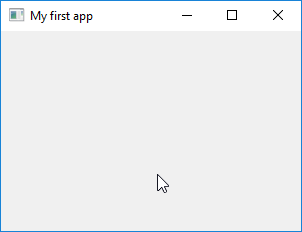
\includegraphics[width=0.4\linewidth]{imgs/myfirstapp.png}}
  \caption{
  Une fenêtre PyQt5 créée par le code \texttt{myfirstapp.py} et également par le code \texttt{myfirstappStructure.py}. \label{fig:myfirstapp}
  }
\end{figure}
%\clearpage % flush figures fig:myfirstapp


\subsection{Structure d'application PyQT}

Les étapes suivantes (dont certaines ont déjà été utilisées dans l'exemple ci-dessus) aideront à créer une structure solide et propre pour toute application développée avec PyQt:

\begin{enumerate}
\item Importer les modules nécessaires.

\item Créer une classe héritée de \texttt{QMainWindow} (à l'aide de la construction \texttt{class MainWindow(QMainWindow):}). La \texttt{QMainWindow} est une classe Qt qui fournit une fenêtre principale de l’application avec toutes les options (telle que la barre de menus, la barre d’état, etc.).

\item Implémentez le \textbf{constructeur} (également appelé \textbf{l'initialiseur}) de la classe en utilisant la méthode \Verb!__init __ ()!. Chaque fois qu'un objet d'une classe est créé, cette méthode sera exécutée. L'initialiseur commence généralement par un appel à l'initialiseur de la classe \texttt{super ()}; Ainsi, toutes les méthodes définies dans la classe parent sont immédiatement disponibles, même si elles sont remplacées dans la définition de classe actuelle.

\item Cette opération est ensuite suivie par la définition des valeurs (par défaut) pour divers attributs, tels que la géométrie, le titre, etc., et la définition des différentes méthodes.

\item Enfin, utiliser la construction \Verb!if __name__ == "__main __":! à la fin pour créer un objet \texttt{QApplication} et l'exécuter.
\end{enumerate}

\noindent
La fenêtre illustrée à la Figure~\ref{fig:myfirstapp} peut également être créée à l'aide des étapes décrites ci-dessus. Le code permettant de faire cela est donné dans le script \textbf{myfirstappStructure.py}. Dans une fenêtre d'invite de commande, exécutez la commande \texttt{python myfirstappStructure.py} (ou exécutez le script sur Spyder), où \textbf{myfirstappStructure.py} est le nom du fichier contenant le code permettant d'afficher la fenêtre illustrée à la Figure~\ref{fig:myfirstapp}.

\begin{pro}{cbg_gray}{bar_gray}\begin{minted}[fontsize=\fontsize{9pt}{9pt},linenos=false,mathescape,baselinestretch=1.0,fontfamily=tt,xleftmargin=2mm]{python}
# NOM DU FICHIER: myfirstappStructure.py
#% IMPORTATION
from PyQt5.QtWidgets import QApplication, QMainWindow

class MainWindow(QMainWindow):
    '''
    DOCUMENTATION
    -------------
    Créer une fenêtre (300x200 pixels)
    '''
    def __init__(self):
        '''
        INITIALISEUR 
        ------------
        La classe `MainWindow()` rendre une fenêtre (300x200 pixels) 
        avec un titre 'My first app'.
        '''
        super(MainWindow, self).__init__()
        # Propriétés de l'interface graphique
        self.setGeometry(400, 100, 300, 200)
        self.setWindowTitle('My first app')

if __name__ == "__main__":
    import sys
    app = QApplication(sys.argv)
    MyApplication = MainWindow()
    MyApplication.show()
    sys.exit(app.exec_())
\end{minted}
\end{pro}
\noindent

\subsection{Widgets, événements et signaux}
Les widgets sont les éléments de base d'une interface graphique. PyQt5 a une large gamme de widgets, y compris des boutons (\texttt{buttons}), des étiquettes (\texttt{labels}), des cases à cocher (\texttt{check boxes}), des curseurs (\texttt{sliders}), des zones de liste (\texttt{list boxes}), etc. Nous décrirons plusieurs widgets couramment utilisés dans cette section. Ceux-ci incluent un \texttt{QPushButton}, un \texttt{ToggleButton}, un \texttt{QLabel}, un \texttt{QCheckBox}, un \texttt{QSlider}, un \texttt{QProgressBar}, un \texttt{QCalendarWidget}, etc.

\paragraph{Ajouter des étiquettes: \texttt{QLabel}.}
Nous avons besoin d'une étiquette pour afficher les messages. Un \texttt{QLabel} peut afficher du texte brut ou riche, HTML. Le code présenté ci-dessous (\textbf{myfirstappLabels.py}) ajouterait deux objets \texttt{QLabel} à la même fenêtre que celle précédemment créée. Le premier affiche un texte brut (\texttt{"Ma première application affiche: "}) et le second un texte HTML enrichi ("Bonjour IE3!", Gras et de couleur verte). L'exécution du code produira une fenêtre illustrée à la Figure~\ref{fig:myfirstappLabels}.
\begin{pro}{cbg_gray}{bar_gray}\begin{minted}[fontsize=\fontsize{9pt}{9pt},linenos=false,mathescape,baselinestretch=1.0,fontfamily=tt,xleftmargin=2mm]{python}
# NOM DU FICHIER: myfirstappLabels.py
#% IMPORTATION
from PyQt5.QtWidgets import QApplication, QMainWindow, QLabel

class MainWindow(QMainWindow):
    '''
    DOCUMENTATION
    -------------
    Créer une fenêtre (300x200 pixels)
    '''
    def __init__(self):
        '''
        INITIALISEUR 
        ------------
        La classe `MainWindow()` rendre une fenêtre (300x200 pixels) 
        avec un titre 'My first app'.
        '''
        super(MainWindow, self).__init__()
        # GUI proprieties
        self.setGeometry(400, 100, 300, 200)
        self.setWindowTitle('My first app')
        # Ajouter des étiquettes: QLabel
        ## Label 1: Texte brut
        label1 = QLabel('Ma première application affiche: ', self)
        # fixer la largeur de l'étiquette
        label1.setFixedWidth(160)
        # position de l'étiquette (x, y) en pixels
        label1.move(10, 10)
        ## Label 2: Texte riche
        label2 = QLabel("", self)
        # créer un message HTML
        message = "<h3><b><font color='green'>Bonjour IE3!</font></b>"
        # ajouter le text du message 
        label2.setText(message)
        # fixer la largeur de l'étiquette
        label2.setFixedWidth(120)
         # position de l'étiquette (x, y) en pixels
        label2.move(200, 10)

if __name__ == "__main__":
    import sys
    app = QApplication(sys.argv)
    MyApplication = MainWindow()
    MyApplication.show()
    sys.exit(app.exec_())
\end{minted}
\end{pro}
\noindent


\begin{figure}[!ht]  % fig:myfirstappLabels
  \centerline{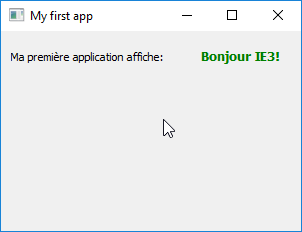
\includegraphics[width=0.4\linewidth]{imgs/myfirstappLabels.png}}
  \caption{
  Résultat de l'exécution du code \texttt{myfirstappLabels.py}. \label{fig:myfirstappLabels}
  }
\end{figure}
%\clearpage % flush figures fig:myfirstappLabels


\paragraph{Ajouter des boutons: \texttt{QPushButton}.}
La plupart des interfaces graphiques sont utilisées pour prendre les entrées de l'utilisateur et produire des sorties en fonction de l'entrée donnée. Une technique courante consiste à demander à l'utilisateur de cliquer sur un bouton \texttt{OK} ou sur un bouton \texttt{Annuler}. Dans PyQt5, cela est implémenté à l'aide de la classe \texttt{QPushButton}. Chaque widget d'une application peut être programmé pour répondre de manière prédéterminée à tout changement survenant dans la fenêtre de l'application ou n'importe où sur l'ordinateur. Ces \emph{changements} sont appelés \textbf{des événements}. Par exemple, nous pourrions déplacer la souris autour de l'écran ou sur la fenêtre de l'application, ou peut-être avons-nous appuyé sur la touche \texttt{Entrée}. Lorsqu'un tel événement se produit, le système émet un ou plusieurs signaux; autrement dit, modifie certaines propriétés des widgets. Nous pouvons écrire du code qui sera exécuté à chaque fois qu'un tel signal est émis. Ce morceau de code s'appelle un \textbf{slot}. Par exemple, nous pouvons souhaiter fermer la fenêtre et quitter l’application lorsque le bouton gauche d’une souris est cliqué sur le bouton de commande \texttt{Annuler}. Lorsque cet événement de clic gauche de la souris sur le bouton \texttt{Annuler} se produit, un signal de \textbf{clicked} est émis sur le bouton et un \textbf{slot} qui quitte l'application et quitte sera implémenté. Cependant, pour que cela se produise, nous devons explicitement \textbf{connecter} le \textbf{slot} au signal. Toutes ces idées sont montrées dans le code \textbf{myfirstappButtons.py}.

\begin{pro}{cbg_gray}{bar_gray}\begin{minted}[fontsize=\fontsize{9pt}{9pt},linenos=false,mathescape,baselinestretch=1.0,fontfamily=tt,xleftmargin=2mm]{python}
# NOM DU FICHIER: myfirstappButtons.py
#% IMPORTATION
from PyQt5.QtWidgets import QApplication, QMainWindow, QLabel, QPushButton
from PyQt5.QtCore import pyqtSlot


class MainWindow(QMainWindow):
    '''
    DOCUMENTATION
    -------------
    Créer une fenêtre (300x200 pixels)
    '''
    def __init__(self):
        '''
        INITIALISEUR 
        ------------
        La classe `MainWindow()` rendre une fenêtre (300x200 pixels) 
        avec un titre 'My first app'.
        '''
        super(MainWindow, self).__init__()
        # GUI proprieties
        self.setGeometry(400, 100, 300, 200)
        self.setWindowTitle('My first app')
        # Ajouter des étiquettes: QLabel
        ## Label 1: Texte brut
        self.label1 = QLabel('Ma première application affiche: ', self)
        # fixer la largeur de l'étiquette
        self.label1.setFixedWidth(160)
        # position de l'étiquette (x, y) en pixels
        self.label1.move(10, 10)
        ## Label 2: Texte riche
        self.label2 = QLabel("", self)
        # créer un message HTML
        message = "<h3><b><font color='green'>Bonjour IE3!</font></b>"
        # ajouter le text du message 
        self.label2.setText(message)
        # fixer la largeur de l'étiquette
        self.label2.setFixedWidth(120)
         # position de l'étiquette (x, y) en pixels
        self.label2.move(200, 10)
        
        # Ajouter des boutons: `QPushButton`
        # Push Button 1: Bouton bonjour
        button1 = QPushButton('Bonjour', self)
        button1.setToolTip("C'est le bouton Bonjour")
        button1.move(50, 50)
        # connecter le signal à l'événement
        button1.clicked.connect(self.on_click_button1)
        # Push Button 2: Bouton au revoir
        button2 = QPushButton('Au revoir', self)
        button2.setToolTip("C'est le bouton Au revoir")
        button2.move(170, 50)
        # connecter le signal à l'événement
        button2.clicked.connect(self.on_click_button2)

    @pyqtSlot()  # signal du bouton bonjour
    def on_click_button1(self):
        '''
        Afficher un message "Bonjour"
        '''
        message = "<h3><b><font color='green'>Bonjour IE3!</font></b>"
        self.label2.setText(message)
        self.label2.setFixedWidth(120)

    @pyqtSlot()  # signal du bouton au revoir
    def on_click_button2(self):
        '''
        Afficher un message "Au revoir"
        '''
        message = "<h3><b><font color='red'>Au revoir IE3!</font></b>"
        self.label2.setText(message)
        self.label2.setFixedWidth(120)

if __name__ == "__main__":
    import sys
    app = QApplication(sys.argv)
    MyApplication = MainWindow()
    MyApplication.show()
    sys.exit(app.exec_())
\end{minted}
\end{pro}
\noindent


\begin{figure}[!ht]  % fig:myfirstappButtons
  \centerline{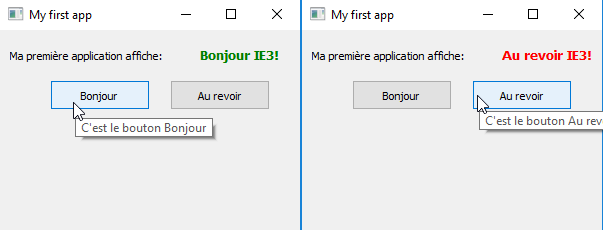
\includegraphics[width=0.4\linewidth]{imgs/myfirstappButtons.png}}
  \caption{
  Résultat de l'exécution du code \texttt{myfirstappButtons.py}. \label{fig:myfirstappButtons}
  }
\end{figure}
%\clearpage % flush figures fig:myfirstappButtons


Toute méthode peut être connectée à un signal. Cependant, pour être sûr, il est préférable de s’assurer qu’une méthode particulière est bien un \textbf{slot}. Ceci est réalisé en déclarant une méthode comme étant un slot en utilisant le décorateur \texttt{@pyqtSlot()} comme indiqué dans le code \textbf{myfirstappButtons.py}.

\paragraph{Ajouter des Spin Box: \texttt{QSpinBox}.}
Les Spin Box sont des widgets utilisés pour accepter et afficher des nombres entiers. Celles-ci peuvent être considérées comme une boîte d'édition avec une molette attachée. En cliquant une fois sur une flèche vers le haut de la molette, la valeur dans la zone d'édition augmente d'un point; cliquer sur la flèche vers le bas diminuera la valeur de un. Vous pouvez également entrer la valeur directement dans la zone d'édition. La plage de valeurs accessible dans un spinbox peut être définie à l'aide de la méthode \texttt{setRange()} ou de la combinaison des méthodes \texttt{setMinimum()} et \texttt{setMaximum()}. Toutes ces idées sont montrées dans le code \textbf{myfirstappSpinBox.py} et illustrées par la Figure~\ref{fig:myfirstappSpinBox}.

\begin{pro}{cbg_gray}{bar_gray}\begin{minted}[fontsize=\fontsize{9pt}{9pt},linenos=false,mathescape,baselinestretch=1.0,fontfamily=tt,xleftmargin=2mm]{python}
# NOM DU FICHIER: myfirstappSpinBox.py
#% IMPORTATION
from PyQt5.QtWidgets import (QApplication, QMainWindow, QLabel,
                             QPushButton, QSpinBox)
from PyQt5.QtCore import pyqtSlot


class MainWindow(QMainWindow):
    '''
    DOCUMENTATION
    -------------
    Créer une fenêtre (300x200 pixels)
    '''
    def __init__(self):
        '''
        INITIALISEUR 
        ------------
        La classe `MainWindow()` rendre une fenêtre (300x200 pixels) 
        avec un titre 'My first app'.
        '''
        super(MainWindow, self).__init__()
        # GUI proprieties
        self.setGeometry(400, 100, 300, 200)
        self.setWindowTitle('My first app')
        # Ajouter des étiquettes: QLabel
        ## Label 1: Texte brut
        self.label1 = QLabel('Ma première application affiche: ', self)
        # fixer la largeur de l'étiquette
        self.label1.setFixedWidth(160)
        # position de l'étiquette (x, y) en pixels
        self.label1.move(10, 10)
        ## Label 2: Texte riche
        self.label2 = QLabel("", self)
        # créer un message HTML
        message = "<h3><b><font color='green'>Bonjour IE3!</font></b>"
        # ajouter le text du message 
        self.label2.setText(message)
        # fixer la largeur de l'étiquette
        self.label2.setFixedWidth(120)
         # position de l'étiquette (x, y) en pixels
        self.label2.move(200, 10)
        
        # Ajouter des boutons: `QPushButton`
        # Push Button 1: Bouton bonjour
        button1 = QPushButton('Bonjour', self)
        button1.setToolTip("C'est le bouton Bonjour")
        button1.move(50, 50)
        # connecter le signal à l'événement
        button1.clicked.connect(self.on_click_button1)
        # Push Button 2: Bouton au revoir
        button2 = QPushButton('Au revoir', self)
        button2.setToolTip("C'est le bouton Au revoir")
        button2.move(170, 50)
        # connecter le signal à l'événement
        button2.clicked.connect(self.on_click_button2)

        # Ajouter des Spin Box: QSpinBox
        self.spb = QSpinBox(self)
        # Spin Box changer une valeur entière de 0 à 100
        self.spb.setMinimum(0)
        self.spb.setMaximum(100)
        self.spb.setValue(50) # valeur par défaut
        self.spb.setSingleStep(1) # pas
        # définir la géométrie (x, y, largeur, hauteur) en pixels
        self.spb.setGeometry(120, 100, 50, 20)
        # connecter le signal à l'événement
        self.spb.valueChanged.connect(self.spb_valuechange)
        # définir une étiquette disant à quoi Spin Box fait référence
        txt = QLabel('La valeur actuelle est: ', self)
        # définir la géométrie (x, y, largeur, hauteur) en pixels
        txt.setGeometry(10, 100, 100, 20)
        # définir une étiquette pour recevoir une valeur du spin box
        self.val = QLabel("", self)
        # définir la géométrie (x, y, largeur, hauteur) en pixels
        self.val.setGeometry(190, 100, 30, 20)

    @pyqtSlot()  # signal du bouton bonjour
    def on_click_button1(self):
        '''
        Afficher un message "Bonjour"
        '''
        message = "<h3><b><font color='green'>Bonjour IE3!</font></b>"
        self.label2.setText(message)
        self.label2.setFixedWidth(120)

    @pyqtSlot()  # signal du bouton au revoir
    def on_click_button2(self):
        '''
        Afficher un message "Au revoir"
        '''
        message = "<h3><b><font color='red'>Au revoir IE3!</font></b>"
        self.label2.setText(message)
        self.label2.setFixedWidth(120)

    @pyqtSlot(int)  # signal du Spin Box: renvoie un entier
    def spb_valuechange(self, value):
        '''
        la valeur du Spin Box est un entier,
        convertissez-le en chaîne à l'aide de la fonction str().
        '''
        self.val.setText(str(self.spb.value()))

if __name__ == "__main__":
    import sys
    app = QApplication(sys.argv)
    MyApplication = MainWindow()
    MyApplication.show()
    sys.exit(app.exec_())
\end{minted}
\end{pro}
\noindent


\begin{figure}[!ht]  % fig:myfirstappSpinBox
  \centerline{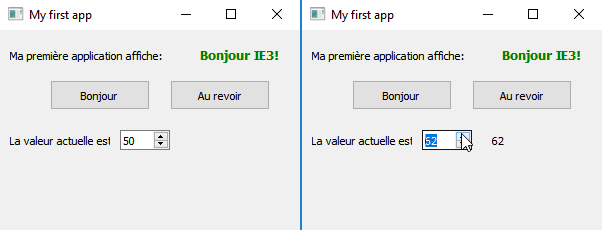
\includegraphics[width=0.4\linewidth]{imgs/myfirstappSpinBox.png}}
  \caption{
  Résultat de l'exécution du code \texttt{myfirstappSpinBox.py}. \label{fig:myfirstappSpinBox}
  }
\end{figure}
%\clearpage % flush figures fig:myfirstappSpinBox


\paragraph{Ajouter des curseurs : \texttt{QSlider}.}
Un QSlider est un widget doté d'une poignée simple. Cette poignée peut être déplacée d'avant en arrière. En utilisant cela, nous pouvons choisir une valeur pour une tâche spécifique. Comme le Spin Box, un curseur ne peut avoir qu'une valeur entière; la plage des valeurs peut être définie entre un minimum et un maximum. Parfois, l’utilisation d’un curseur est plus naturelle que celle d’un Spin Box et cela dépend de la tâche ou de l’application.

\begin{pro}{cbg_gray}{bar_gray}\begin{minted}[fontsize=\fontsize{9pt}{9pt},linenos=false,mathescape,baselinestretch=1.0,fontfamily=tt,xleftmargin=2mm]{python}
# NOM DU FICHIER: myfirstappSlider.py
#% IMPORTATION
from PyQt5.QtWidgets import (QApplication, QMainWindow, QLabel,
                             QPushButton, QSpinBox, QSlider)
from PyQt5.QtCore import pyqtSlot, Qt


class MainWindow(QMainWindow):
    '''
    DOCUMENTATION
    -------------
    Créer une fenêtre (300x200 pixels)
    '''
    def __init__(self):
        '''
        INITIALISEUR 
        ------------
        La classe `MainWindow()` rendre une fenêtre (300x200 pixels) 
        avec un titre 'My first app'.
        '''
        super(MainWindow, self).__init__()
        # GUI proprieties
        self.setGeometry(400, 100, 300, 200)
        self.setWindowTitle('My first app')
        # Ajouter des étiquettes: QLabel
        ## Label 1: Texte brut
        self.label1 = QLabel('Ma première application affiche: ', self)
        # fixer la largeur de l'étiquette
        self.label1.setFixedWidth(190)
        # position de l'étiquette (x, y) en pixels
        self.label1.move(10, 10)
        ## Label 2: Texte riche
        self.label2 = QLabel("", self)
        # créer un message HTML
        message = "<h3><b><font color='green'>Bonjour IE3!</font></b>"
        # ajouter le text du message 
        self.label2.setText(message)
        # fixer la largeur de l'étiquette
        self.label2.setFixedWidth(120)
         # position de l'étiquette (x, y) en pixels
        self.label2.move(200, 10)
        
        # Ajouter des boutons: `QPushButton`
        # Push Button 1: Bouton bonjour
        button1 = QPushButton('Bonjour', self)
        button1.setToolTip("C'est le bouton Bonjour")
        button1.move(50, 50)
        # connecter le signal à l'événement
        button1.clicked.connect(self.on_click_button1)
        # Push Button 2: Bouton au revoir
        button2 = QPushButton('Au revoir', self)
        button2.setToolTip("C'est le bouton Au revoir")
        button2.move(170, 50)
        # connecter le signal à l'événement
        button2.clicked.connect(self.on_click_button2)

        # Ajouter des Spin Box: QSpinBox
        self.spb = QSpinBox(self)
        # Spin Box changer une valeur entière de 0 à 100
        self.spb.setMinimum(0)
        self.spb.setMaximum(100)
        self.spb.setValue(50) # valeur par défaut
        self.spb.setSingleStep(1) # pas
        # définir la géométrie (x, y, largeur, hauteur) en pixels
        self.spb.setGeometry(120, 100, 50, 20)
        # connecter le signal à l'événement
        self.spb.valueChanged.connect(self.spb_valuechange)
        # définir une étiquette disant à quoi Spin Box fait référence
        txt = QLabel('La valeur actuelle est: ', self)
        # définir la géométrie (x, y, largeur, hauteur) en pixels
        txt.setGeometry(10, 100, 100, 20)
        # définir une étiquette pour recevoir une valeur du spin box
        self.val = QLabel("", self)
        # définir la géométrie (x, y, largeur, hauteur) en pixels
        self.val.setGeometry(190, 100, 30, 20)

        # Slider: Slider change integer value from 0 to 100
        self.sldr = QSlider(Qt.Horizontal, self)
        self.sldr.setMinimum(0)
        self.sldr.setMaximum(100)
        self.sldr.setValue(50)
        self.sldr.setSingleStep(1)
        # set geometry (x,y,width,hight)
        self.sldr.setGeometry(10, 150, 280, 20)
        self.sldr.valueChanged.connect(self.sldr_valuechange)

    @pyqtSlot()  # signal du bouton bonjour
    def on_click_button1(self):
        '''
        Afficher un message "Bonjour"
        '''
        message = "<h3><b><font color='green'>Bonjour IE3!</font></b>"
        self.label2.setText(message)
        self.label2.setFixedWidth(120)

    @pyqtSlot()  # signal du bouton au revoir
    def on_click_button2(self):
        '''
        Afficher un message "Au revoir"
        '''
        message = "<h3><b><font color='red'>Au revoir IE3!</font></b>"
        self.label2.setText(message)
        self.label2.setFixedWidth(120)

    @pyqtSlot(int)  # signal du Spin Box: renvoie un entier
    def spb_valuechange(self, value):
        '''
        la valeur du Spin Box est un entier,
        convertissez-le en chaîne à l'aide de la fonction str().
        '''
        self.val.setText(str(self.spb.value()))
        # connecter le curseur au Spin Box
        self.sldr.setValue(value)

    @pyqtSlot(int)  # signal du curseur
    def sldr_valuechange(self, value):
        '''
        connecter le Spin Box au curseur
        '''
        self.spb.setValue(value)


if __name__ == "__main__":
    import sys
    app = QApplication(sys.argv)
    MyApplication = MainWindow()
    MyApplication.show()
    sys.exit(app.exec_())
\end{minted}
\end{pro}
\noindent


\begin{figure}[!ht]  % fig:myfirstappSlider
  \centerline{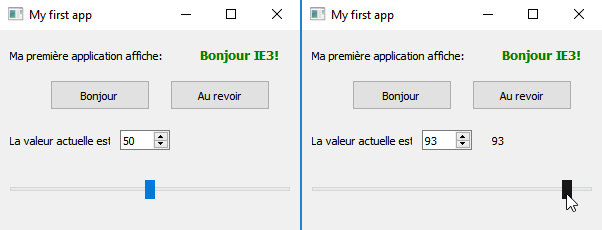
\includegraphics[width=0.4\linewidth]{imgs/myfirstappSlider.png}}
  \caption{
  Résultat de l'exécution du code \texttt{myfirstappSlider.py}. \label{fig:myfirstappSlider}
  }
\end{figure}
%\clearpage % flush figures fig:myfirstappSlider


\section{Le concepteur Qt: "Qt Designer"}
Le paquet PyQt est livré avec un outil de générateur d'interface graphique appelé Qt Designer (ou concepteur Qt). Qt Designer est l’outil Qt permettant de concevoir et de construire des interfaces graphiques à l’aide d’une simple approche \textbf{glisser-déposer}. Il vous permet de concevoir des widgets, des boîtes de dialogue ou des fenêtres principales complètes à l'aide de formulaires à l'écran (en anglais appelés: on-screen forms). Il a la possibilité de prévisualiser les conceptions pour s'assurer que l'interface graphique fonctionne comme prévu. Il permet une interface de prototypage avant qu’un code ne soit écrit.

Qt Designer peut être démarré en tapant \texttt{designer} dans la fenêtre d'invite de commande sous Windows ou sur un terminal sous n'importe quel système Linux. Sur un Mac, double-cliquez sur l'application Qt Desginer dans le répertoire "anaconda3 / bin" pour lancer Qt Designer. Une fois démarré, Qt Designer ressemblera à celui illustré à la figure~\ref{fig:designerNew}.

La création d’une interface graphique à l’aide de Qt Designer commence par la sélection d’une fenêtre de niveau supérieur pour l’application. Dans un premier temps, Qt Designer affiche une boîte de dialogue d’initialisation dans laquelle vous pouvez choisir le type de base de l’interface graphique que vous souhaitez créer. Vous avez la possibilité de choisir entre trois types de formulaires: \textbf{Dialog}, \textbf{Main Window} et \textbf{Widget}.


\begin{figure}[!ht]  % fig:designerNew
  \centerline{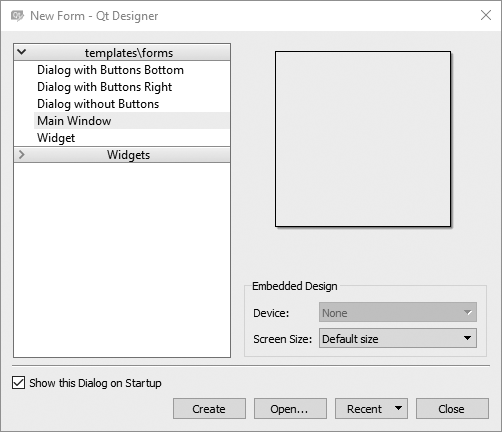
\includegraphics[width=0.7\linewidth]{imgs/designerNew.png}}
  \caption{
  Dialogue d'initialisation du concepteur Qt. \label{fig:designerNew}
  }
\end{figure}
%\clearpage % flush figures fig:designerNew


Une fois que le type de formulaire requis est sélectionné et créé (en cliquant sur le bouton \textbf{Create}), il peut être redimensionné pour répondre aux besoins de l'application et tous les widgets peuvent être placés dessus.

\subsection{La fenêtre du concepteur Qt}
Par défaut, à gauche du formulaire se trouve un panneau appelé la \emph{Boîte à widgets} (Widget Box) qui contient tous les objets Qt regroupés sous différentes catégories. Sur la droite, de nombreux panneaux tels que \emph{l'inspecteur d'objets} (Object Inspector), \emph{l'éditeur de propriétés} (Property Editor), etc.


\begin{figure}[!ht]  % fig:designerWindow
  \centerline{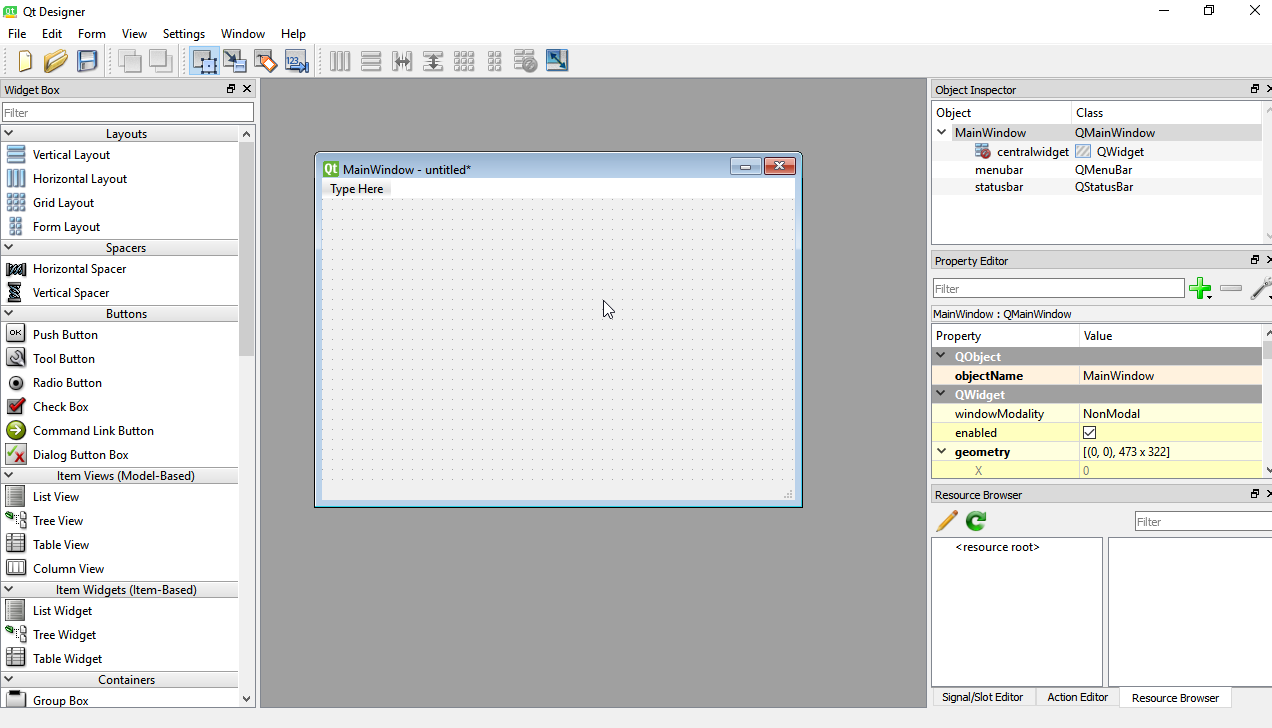
\includegraphics[width=0.9\linewidth]{imgs/designerWindow.png}}
  \caption{
  La fenêtre du concepteur Qt. \label{fig:designerWindow}
  }
\end{figure}
%\clearpage % flush figures fig:designerWindow


\subsection{L'éditeur de propriété}

Nous pouvons choisir le widget souhaité dans la \textbf{Boîte des widgets}, le faire glisser et le déposer sur le formulaire Qt, puis modifier ses propriétés à l'aide de \textbf{l'éditeur de propriétés}. Par exemple, faisons glisser deux widgets de la catégorie \textbf{Display Widgets}  dans la Boîte des widgets. Chaque widget a la propriété commune appelée \textbf{objectName} dont les valeurs peuvent être définies dans l'éditeur de propriétés. Par exemple, dans notre cas, \texttt{label} et \Verb!label_2! sont les objectName par défaut des deux labels ajouté à l'interface que nous allons changé par \texttt{label1} et \texttt{label2} respectivement. On peut changer le texte de ces labels en cliquant deux fois sur le texte par défaut ou en cliquant sur \texttt{<Bouton droite Modifier texte simple/texte riche>}. La vidéo ci dessous illustre les étape de création de l'interface graphique "My first app" avec le concepteur Qt.

\begin{notice_grayiconadmon}[Notice]
Une fois que tous les widgets sont définis dans la position souhaitée et que les valeurs des différentes propriétés de tous les widgets sont définies, nous pouvons examiner comment la fenêtre de l'interface graphique ressemblerait par prévisualisation. Cela se fait en tapant \texttt{<Ctrl + R>} sur le clavier.
\end{notice_grayiconadmon} % title: Notice




\begin{doconce:movie}
\refstepcounter{doconce:movie:counter}
\begin{center}
\href{{https://www.youtube.com/watch?v=YSeyRZXOfuk}}{\nolinkurl{https://www.youtube.com/watch?v=YSeyRZXOfuk}}
\end{center}

\begin{center}  % movie caption
Movie \arabic{doconce:movie:counter}: YouTube movie.
\end{center}
\end{doconce:movie}




\begin{figure}[!ht]  % fig:myfirstappDesigner
  \centerline{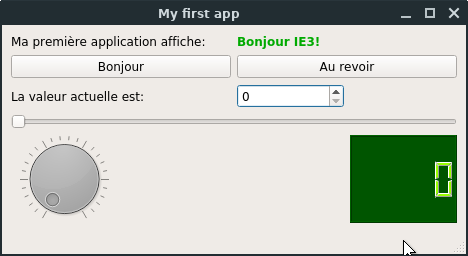
\includegraphics[width=0.4\linewidth]{imgs/myfirstappDesigner.png}}
  \caption{
  Interface graphique créée par le concepteur Qt. \label{fig:myfirstappDesigner}
  }
\end{figure}
%\clearpage % flush figures fig:myfirstappDesigner


% ------------------- end of main content ---------------

% #ifdef PREAMBLE
\end{document}
% #endif

